\chapter{Cost-benefit considerations in the growth of spatial networks}
\label{chap:cost-benefit}


Our societies rely on various networks for the distribution of energy,
information and for transportation of individuals. These networks shape the
spatial organization of our societies and their understanding is a key step
towards the understanding of the characteristics and the evolution of our
cities~\cite{Batty:2013}. Despite their apparent diversity, these networks are
all particular examples of a broader class of networks --spatial networks--
which are characterised by the embedding of their nodes in space. As a
consequence, there is usually a cost associated with a link, leading to
particular structures which are now fairly well
understood~\cite{Barthelemy:2011}, thanks to the recent availability of large
sets of data. Nevertheless, the mechanisms underlying the formation and temporal
evolution of spatial networks have not been much studied. Different kinds of
models aiming at explaining the static characteristics of spatial networks have
been suggested previously in quantitative geography, transportation economics,
and physics (for a review, see ~\cite{Xie:2009}). Concerning the time
evolution of spatial networks, a few models only exist to describe in particular
the growth of road and rail networks~\cite{Levinson:2006, Gastner:2006,
Barthelemy:2008, Courtat:2011}, but a general framework is yet to be
discovered.\\


The earliest attempts can be traced back to the economic geography community in
the 60s and 70s (A fairly comprehensive review of these studies can be found
in~\cite{Haggett:1969}). However, due to the lack of available data and
computational power, most of the proposed models were based on intuitive,
heuristic rules and have not been studied thoroughly. Interestingly,
\cite{Black:1971} attempts to reproduce railway networks with the same
cost-benefits approach that will be adopted in the following.

A more recent trend is that of the optimization models. The common point between
all these models is that they try to reproduce the topological features of
existing networks, by considering the network as the realisation of the optimum
of given quantity (see section IV.E in~\cite{Barthelemy:2011} for an overview).
For instance, the hub-and-spoke models~\cite{OKelly:1998} reproduce correctly
with an optimization procedure the observed hierarchical organization of city
pair relations. However, the vast majority of the existing spatial networks do
not seem to result from a global optimization, but rather from the progressive
addition of nodes and segments resulting from a local optimization. By modeling
(spatial) networks as resulting from a global optimization, one overlooks the
usually limited time horizon of planners and the self-organization underlying
their formation.

Self-organization of transportation networks has already been studied in
transportation engineering~\cite{Levinson:2006, Xie:2009}. Using an agent-based
model including various economical ingredients, the authors
of~\cite{Levinson:2006} modeled the emergence of the networks properties as a
degeneration process. Starting from an initial grid, traffics are computed at
each time step and each edge computes its costs and benefits accordingly, using
any excess to improve their speed. After several iterations, a hierarchy of
roads emerges. Our approach is very different: we start from nodes and we do not
specify any initial network. Also, and most importantly, we deliberately do not
represent all the causal mechanisms at work in the system. Indeed, the aim of
our model is to understand the basic ingredients for emergence of patterns that
can be observed in various systems and we thus focus on a single, very general
economical mechanism and its consequence on the large-scale properties of the
networks.

Concerning spatial networks, as it is the case for many spatial structure, there
is a strong path dependency. In other words, the properties of a network at a
certain time can be explained by the particular historical path leading to it.
It thus seems reasonable to model spatial networks in an iterative way. Some
iterative models, following ideas for understanding power laws in the Internet
\cite{Fabrikant:2002} and describing the growth of transportation
networks~\cite{Gastner:2006} can be found in the literature. In these models,
the graphs are constructed via an iterative greedy optimization of geometrical
quantities. However, we believe that the topological and geometrical properties
of networks are consequences of the underlying processes at stake. At best,
geometrical and topological quantities can be a proxy for other --more
fundamental-- properties: for instance, it will be clear in what follows that
the length of an edge can be taken as a proxy for the cost associated with the
existence of that edge. Finding those underlying processes is a key step towards
a general framework within which the properties of networks can be understood
and, hopefully, predicted.\\

In this respect, cost-benefit analysis (CBA) provides a systematic method to
evaluate the economical soundness of a project. It allows one to appreciate
whether the costs of a decision will outweigh its benefits and therefore
evaluate quantitatively its feasibility and/or suitability. Cost-benefit
analysis has only been officially used to assess transport investments since
1960~\cite{Coburn:1960}. However, the concept comes accross as so intuitive in
our profit-driven economies that it seems reasonable to wonder whether CBA is at
the core of the emergent features of our societies such as distribution and
transportation systems. If the temporal evolution of spatial networks is rarely
studied, arguments mentioning the costs and benefits related to such networks
are almost absent from the physics litterature (\cite{Popovic:2012} is a notable
exception, although they do not consider the time evolution of the network.).
However, we find it intuitively appealing that in an iterative model, the
formation of a new link should --at least locally-- correspond to a cost-benefit
analysis. We therefore propose here a simple cost-benefit analysis framework for
the formation and evolution of spatial networks. Our main goal within this
approach is to understand the basic processes behind the self-organization of
spatial networks that lead to the emergence of their large scale properties.




\section{The model}

\subsection{Theoretical formulation}
\label{sub:theoretical_formulation}

We consider here the simple case where all the nodes are distributed uniformly
in the plane (see Methods for detailed description of the algorithm). For a rail
network, the nodes would correspond to cities and the network grows by adding
edges between cities iteratively; the edges are added sequentially to the graph
--as a result of a cost-benefit analysis-- until all the nodes are connected.
For the sake of simplicity, we limit ourselves to the growth of trees which
allows to focus on the emergence of large-scale structures due to the
cost-benefit ingredient alone.  Furthermore, we consider that all the actors
involved in the building process are perfectly rational and therefore that the
most profitable edge is built at each step. More precisely, at each time step we
build the link connecting a new node $i$ to a node $j$ which already belongs to
the network, such that the following quantity is maximum

\begin{equation}
    R_{ij} = B_{ij} - C_{ij}
    \label{eq:general_framework}
\end{equation}

The quantity $B_{ij}$ is the \textit{expected benefit} associated with the
construction of the edge between node $i$ and node $j$ and $C_{ij}$ is the
\textit{expected cost} associated with such a construction. Eq.
(\ref{eq:general_framework}) defines the general framework of our model and we
now discuss specific forms of $R_{ij}$. In the case of transportation networks,
the cost will essentially correspond to some maintenance cost and will typically
be proportional to the euclidean distance $d_{ij}$ between $i$ and $j$. We thus
write

\begin{equation}
    C_{ij} = \kappa d_{ij}
    \label{eq:cost}
\end{equation}

where $\kappa$ represents the cost of a line per unit of length per unit of
time. Benefits are more difficult to assess. For rail networks, a simple yet
reasonable assumption is to write the benefits in terms of distance and expected
traffic $T_{ij}$ between cities $i$ and $j$ 

\begin{equation} 
    B_{ij} = \eta T_{ij} d_{ij}
    \label{eq:benefits} 
\end{equation}

where $\eta$ represents the benefits per passenger per unit of length. We have
to estimate the expected traffic between two cities and for this we will follow
the common and simple assumption used in the transportation litterature, of
having the so-called gravity law ~\cite{Stewart:1948,Erlander:1990}

\begin{equation} 
    T_{ij} = k\frac{M_i \: M_j}{d_{ij}^a} 
    \label{eq:gravity} 
\end{equation}

where $M_{i(j)}$ is the population of city $i(j)$, and $k$ is the rate
associated with the process. We will choose here a value of the exponent $a>1$
($a<1$ would correspond to an unrealistic situation where the benefits
associated with passenger traffic would increase with the distance). This
parameter $a$ determines the range at which a given city attracts traffic,
regardless of the density of cities. The accuracy and relevance of this gravity
law is still controversial and improvements have been recently
proposed~\cite{Simini:2012,Lenormand:2012}. But it has the advantage of being
simple and to capture the essence of the traffic phenomenon: the decrease of the
traffic with distance and the increase with population. Within these
assumptions, the cost-benefit budget $R'_{ij}=R_{ij}/\eta$ now reads
\begin{equation} \label{eq:R0} R'_{ij} = k\frac{M_i M_j}{d_{ij}^{\;a-1}} - \:
\beta d_{ij} \end{equation} where $\beta = \frac{\kappa}{\eta}$ represents the
relative importance of the cost with regards to the benefits. We will assume
that populations are power-law distributed with exponent $\mu$ (which for cities
is approximatively $\mu\approx 1.1$, see Methods) and the model thus depends
essentially on the two parameters $a$, and $\beta$ (for a detailed description
of parameter used in this paper, see the next section). In the following we will
be working with fixed values of $\mu$ and $a$. The exact values we choose are
however not important as the obtained graphs would have the same qualitative
properties.


\subsection{Simulations} 

The simulation starts by distributing nodes uniformly in a square. We then
attribute to each node a random population distributed according to the power
law

\begin{equation}
    P_M(x) = \frac{\mu}{x^{\mu+1}}
\end{equation}

The choice of this distribution is motivated by Zipf's empirical results on city
populations~\cite{Zipf:1949} (which motivates the choice $\mu=1.1$ in our
simulations) but also because we can go from a peaked to a broad distribution by
tuning the value of $\mu$. Indeed, for $\mu>2$, both the first and the second
moment of this distribution exist and the distribution can be considered as
peaked. In contrast for $1<\mu<2$, only the first moment converges and the
distribution is broad.

Once the set of nodes is generated, we choose a random node as the root and add
nodes recursively until all the nodes belong to the graph. At each time step,
the nodes belonging to the graph constitute the set of `inactive nodes', and the
other -not yet connected - nodes the `active' nodes. At each time step we
connect an active node to an inactive node such that their value of $R$ defined
in Eq.~\ref{eq:R0} is maximum.




\section{Crossover between star-graph and Minimum Spanning Tree}

\subsection{Typical scale} 

The average population is $\overline{M}$ and the typical inter-city distance is
given by $\ell_1\sim 1/\sqrt{\rho}$ where $\rho=N/L^2$ denotes the city density
($L$ is the typical size of the whole system). The two terms of Eq.~\ref{eq:R0}
are thus of the same order for $\beta=\beta^*$ defined as

\begin{equation}
    \beta^* = k \overline{M}^2 \rho^{a/2}
    \label{eq:beta*}
\end{equation}

In the theoretical discussion that follows, we will take $k=1$ for simplicity
(but it should not be forgotten in empirical discussions). Another way of
interpreting $\beta^*$ which makes it more practical to estimate from empirical
data (see section Discussion), is to say that it is of the order of the average
traffic per unit time

\begin{equation} 
    \beta^* = < T > 
    \label{eq:beta*_traffic} 
\end{equation}

From Eq.~\ref{eq:beta*} we can guess the existence of two different regimes
depending on the value of $\beta$:

\begin{itemize}
    \item $\beta \ll \beta^*$ the cost term is negligible compared to the
    benefits term. Each connected city has its own influence zone depending on
its population and the new cities will tend to connect to the most influent
city. In the case where $a\approx 1$, every city connects to the most populated
cities and we obtain a star graph constituted of one single hub connected to all
other cities.  
    \item $\beta \gg \beta^*$ the benefits term is negligible
    compared to the cost term. All new cities will connect sequentially to their
    closest neighbour. Our algorithm is then equivalent to an implementation of
    Prim's algorithm~\cite{Prim:1957}, and the resulting graph is a minimum
    spanning tree (MST).  
\end{itemize}

The intermediate regime $\beta\simeq\beta^*$ however needs to be elucidated.  In
particular, we have to study if there is a transition or a crossover between the
two extreme network structures, and if we have a crossover what is the network
structure in the intermediate regime. In the following we answer these questions
by simulating the growth of these spatial networks.


\subsection{Evidence for the crossover}

Fig.~\ref{fig:plot_graphs} shows three graphs obtained for the same set of
cities for three different values of $\beta/\beta^*$ ($a=1.1$, $\mu=1.1$)
confirming our discussion about the two extreme regimes in the previous section.
A visual inspection seems to show that for $\beta \sim \beta^*$ a different type
of graph appears, which suggests the existence of a crossover between the
star-graph and the MST. This graph is reminiscent of the hub-and-spoke structure
that has been used to describe the interactions between city
pairs~\cite{OKelly:1998,OKelly:1996}. However, in contrast with the rest of the
literature about hub-and-spoke models, we show that this structure is not
necessarily the result of a global optimization: indeed, it emerges here as the
result of the auto-organization of the system.

\begin{figure}
    \centering
    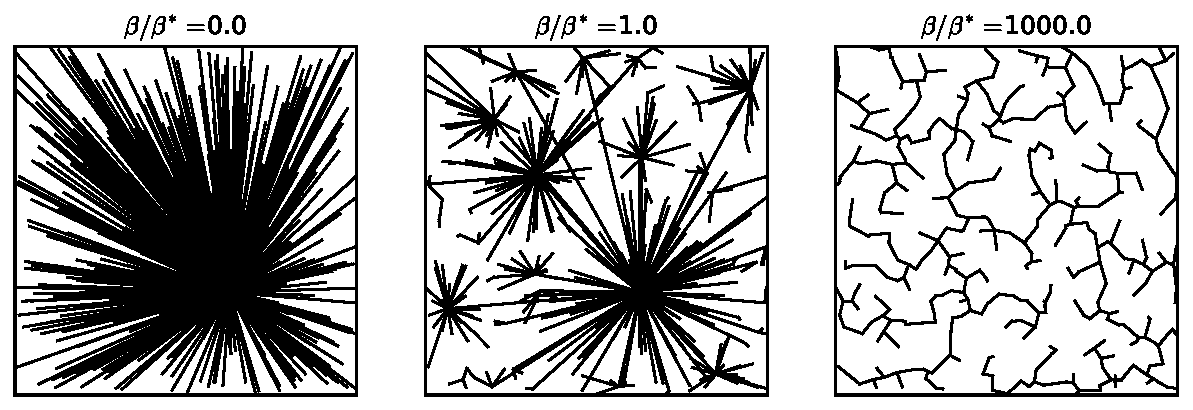
\includegraphics[width=\textwidth]{gfx/chapter-networks/figure1.pdf}
    \caption{{\bf Simulated graphs.} Graphs obtained with our algorithm for the same set of cities
    (nodes) for three different values of $\beta^*$ ($a=1.1$, $\mu=1.1$, $400$
cities). On the left panel, we have a star graph where the most populated node
is the hub and on the right panel, we recover the minimum spanning tree.
\label{fig:plot_graphs}} 
\end{figure}

The MST is characterised by a peaked degree distribution while the star graph's
degree distribution is bimodal, and we therefore choose to monitor the crossover
with the Gini coefficient for the degrees defined as in~\cite{Dixon:1987}

\begin{equation}
    G_k = \frac{1}{2 N^2 \bar{k}} \sum_{i,j=1}^{N} | k_i - k_j |
    \label{eq:gini}
\end{equation}

where $\bar{k}$ is the average degree of the network. The Gini coefficient is in
$[0,1]$ and if all the degrees are equal, it is easy to see that $G=0$. On the
other hand, if all nodes but one are of degree 1 (as in the star-graph), a
simple calculation shows that $G=1/2$. Fig.~\ref{fig:gini} displays the
evolution of the Gini coefficient versus $\beta/\beta^*$ (for different values
of $\beta^*$ obtained by changing the value of $a$, $\mu$ and $N$). This plot
shows a smooth variation of the Gini coefficient pointing to a crossover between
a star graph and the MST,  as one could expect from the plots on
Fig.~\ref{fig:plot_graphs} (also, we note that for given values of $a$, $\mu$
all the plots collapse on the same curve, regardless of the number $N$ of nodes.
However for different values of $a$ or $\mu$ we obtain different curves).

\begin{figure}
    \centering
    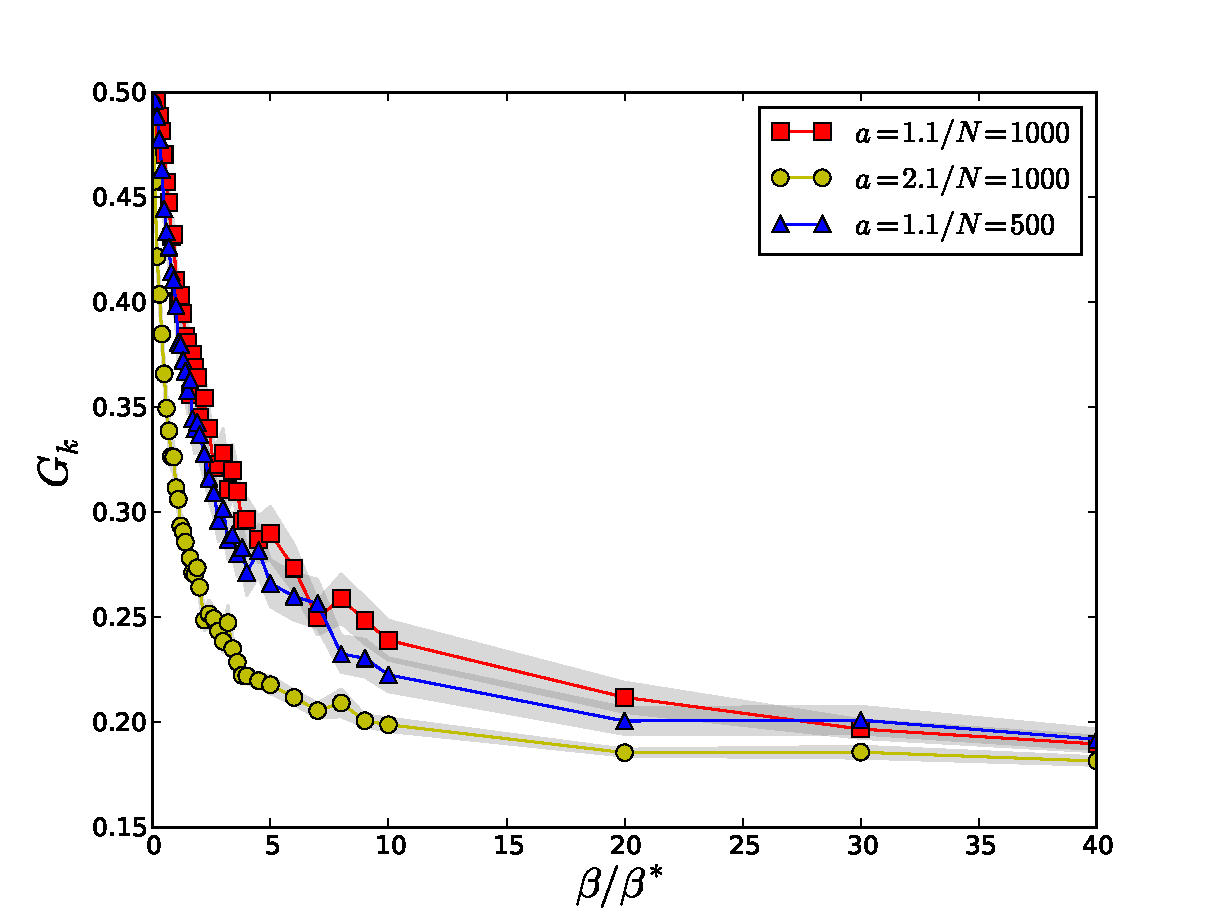
\includegraphics[width=0.8\textwidth]{gfx/chapter-networks/figure2.pdf}
    \caption{{\bf Gini on node degrees.} Evolution of the Gini coefficient with
$\beta/\beta^*$ for different values of $\beta^*$. The shaded area represents
the standard deviation of the Gini coefficient. Values decrease from $0.5$ in
the star-graph regime to below $0.20$ in the MST regime.\label{fig:gini}} \end{figure}

Another important difference between the star-graph and the MST lies in how the
total length of the graph scales with its number of nodes. Indeed, in the case
of the star-graph, all the nodes are connected to the same node and the typical
edge length is $L$, the typical size of the system the nodes are enclosed in. We
thus obtain

\begin{equation}
    L_{tot} \sim L\; N
    \label{eq:Ltot_star}
\end{equation}

On the other hand, for the MST each node is connected roughly to its nearest
neighbour at distance typically given by $\ell_1\sim L/\sqrt{N}$, leading to

\begin{equation}
    L_{tot} \sim L\; \sqrt{N}
    \label{eq:Ltot_MST}
\end{equation}

More generally, we expect a scaling of the form $L_{tot}\sim N^\tau$ and on
Fig.~\ref{fig:Ltot_vs_beta} we show the variation of the exponent $\tau$ versus
$\beta$. For $\beta=0$ we have $\tau=1.0$ and we recover the behavior $L_{tot}
\propto N$ typical of a star graph. In the limit $\beta \gg \beta^*$ we also
recover the scaling $L_{tot} \propto \sqrt{N}$, typical of a MST. For
intermediate values, we observe an exponent which varies continuously in the
range $[0.5,1.0]$. This rather surprising behavior is rooted in the
heterogeneity of degrees and in the following, we will show that we can
understand this behaviour as resulting from the hierarchical structure of the
graphs in the intermediate regime. 

\begin{figure}
    \centering
    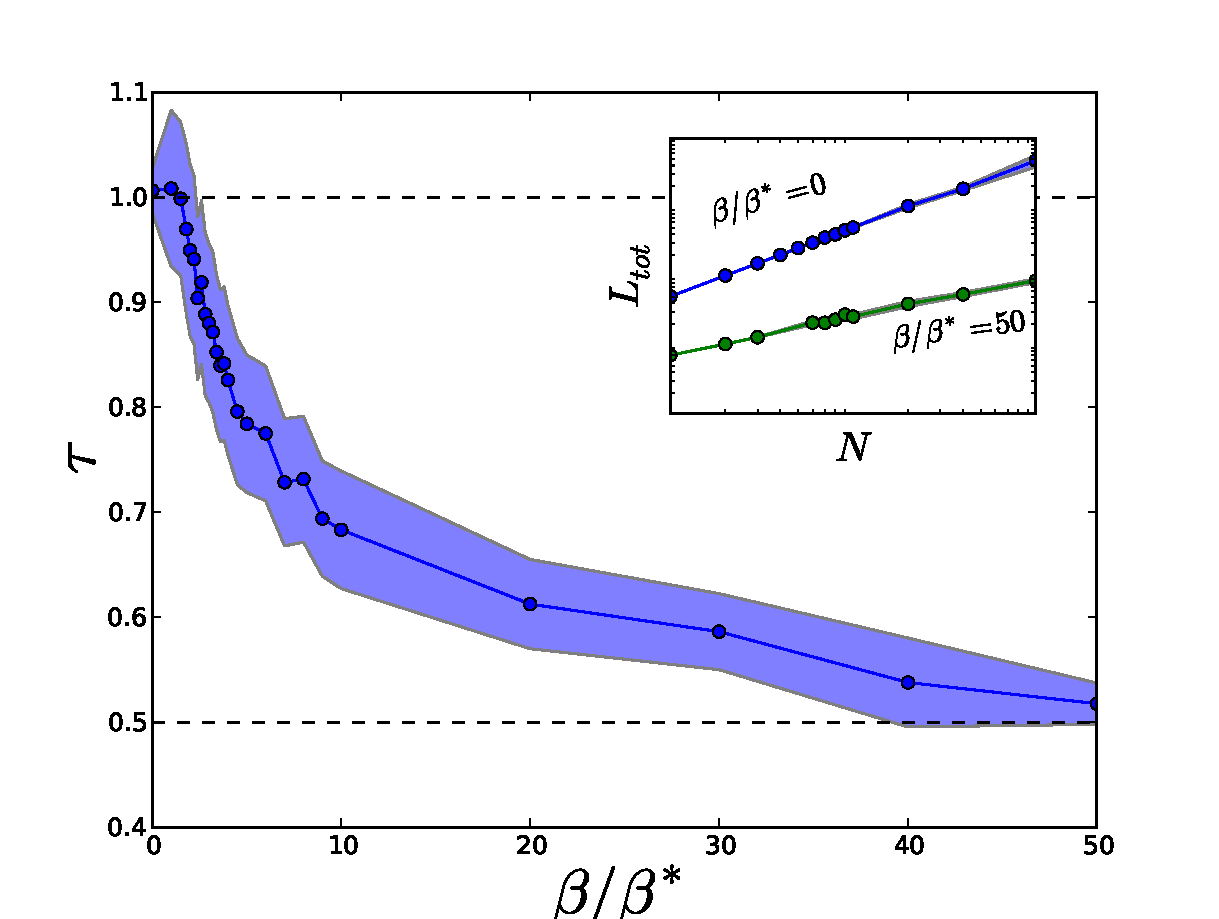
\includegraphics[width=\textwidth]{gfx/chapter-networks/figure3.pdf} 
    \caption{{\bf Star graph to MST transition.} Exponent $\tau$ versus $\beta$.
For $\beta\ll \beta^*$ we recover the star-graph exponent $\tau=1$ and for the
other extreme $\beta\gg\beta^*$ we recover the MST exponent $\tau=1/2$. In the
intermediate range, we observe a continuously varying exponent suggesting a
non-trivial structure. The shaded area represents the standard deviation of
$\tau$.\label{fig:Ltot_vs_beta}. (Inset) In order to illustrate how we determined
the value of $\tau$, we represent $L_{tot}$ versus $N$ for two different values
of $\beta$. The power law fit of these curves gives $\tau$.} 
\end{figure}

It is interesting to note that a scaling with an exponent $1/2<\tau < 1$ has
been observed~\cite{Samaniego:2008,Barthelemy:2011} for the total number
$\ell_T$ of miles driven by the population (of size $P$) of city scales as
$\ell_T \propto P^{\beta}$ with $\beta=0.66$. Understanding the origin of those
intermediate numbers might thus also give us insights into important features of
traffic in urban areas and the structure of cities.

It thus seems that from the point of view of interesting quantities such as the
Gini coefficient or the exponent $\tau$, there is no sign of a critical value
for $\beta$ and that we are in presence of a crossover and not a transition.


\section{Spatial Hierarchy}

The graph corresponding to the intermediate regime $\beta \approx \beta^*$
depicted on Fig.~\ref{fig:plot_graphs} exhibits a particular structure
corresponding to a hierarchical organization, observed in many complex
networks~\cite{Sales-Pardo:2007}. Inspired from the observation of networks in
the regime $\beta/\beta^* \sim 1$, we define a particular type of hierarchy
--that we call \emph{spatial hierarchy}-- as follows. A network will be said to
be spatially hierarchical if:

\begin{enumerate}
    \item  We have a hierarchical network of hubs that connect to nodes less and less far away as one goes down the hierarchy;
    \item Hubs belonging to the same hierarchy level have their own influence zone clearly separated from the others'. In addition, the influence zones of a given level are included in the influence zones of the previous level.
\end{enumerate} 

The relevance of this new concept of hierarchy in the present context can be
qualitatively assessed on Fig.~\ref{fig:separation_example} where we represent
the influence zones by colored circles, the colors corresponding to different
hierarchical levels. In order to go beyond this simple, qualitative description
of the structure, we provide in the following a quantitative proof that networks
in the regime $\beta / \beta^*$ exhibit spatial hierarchy.

\begin{figure} 
    \centering
    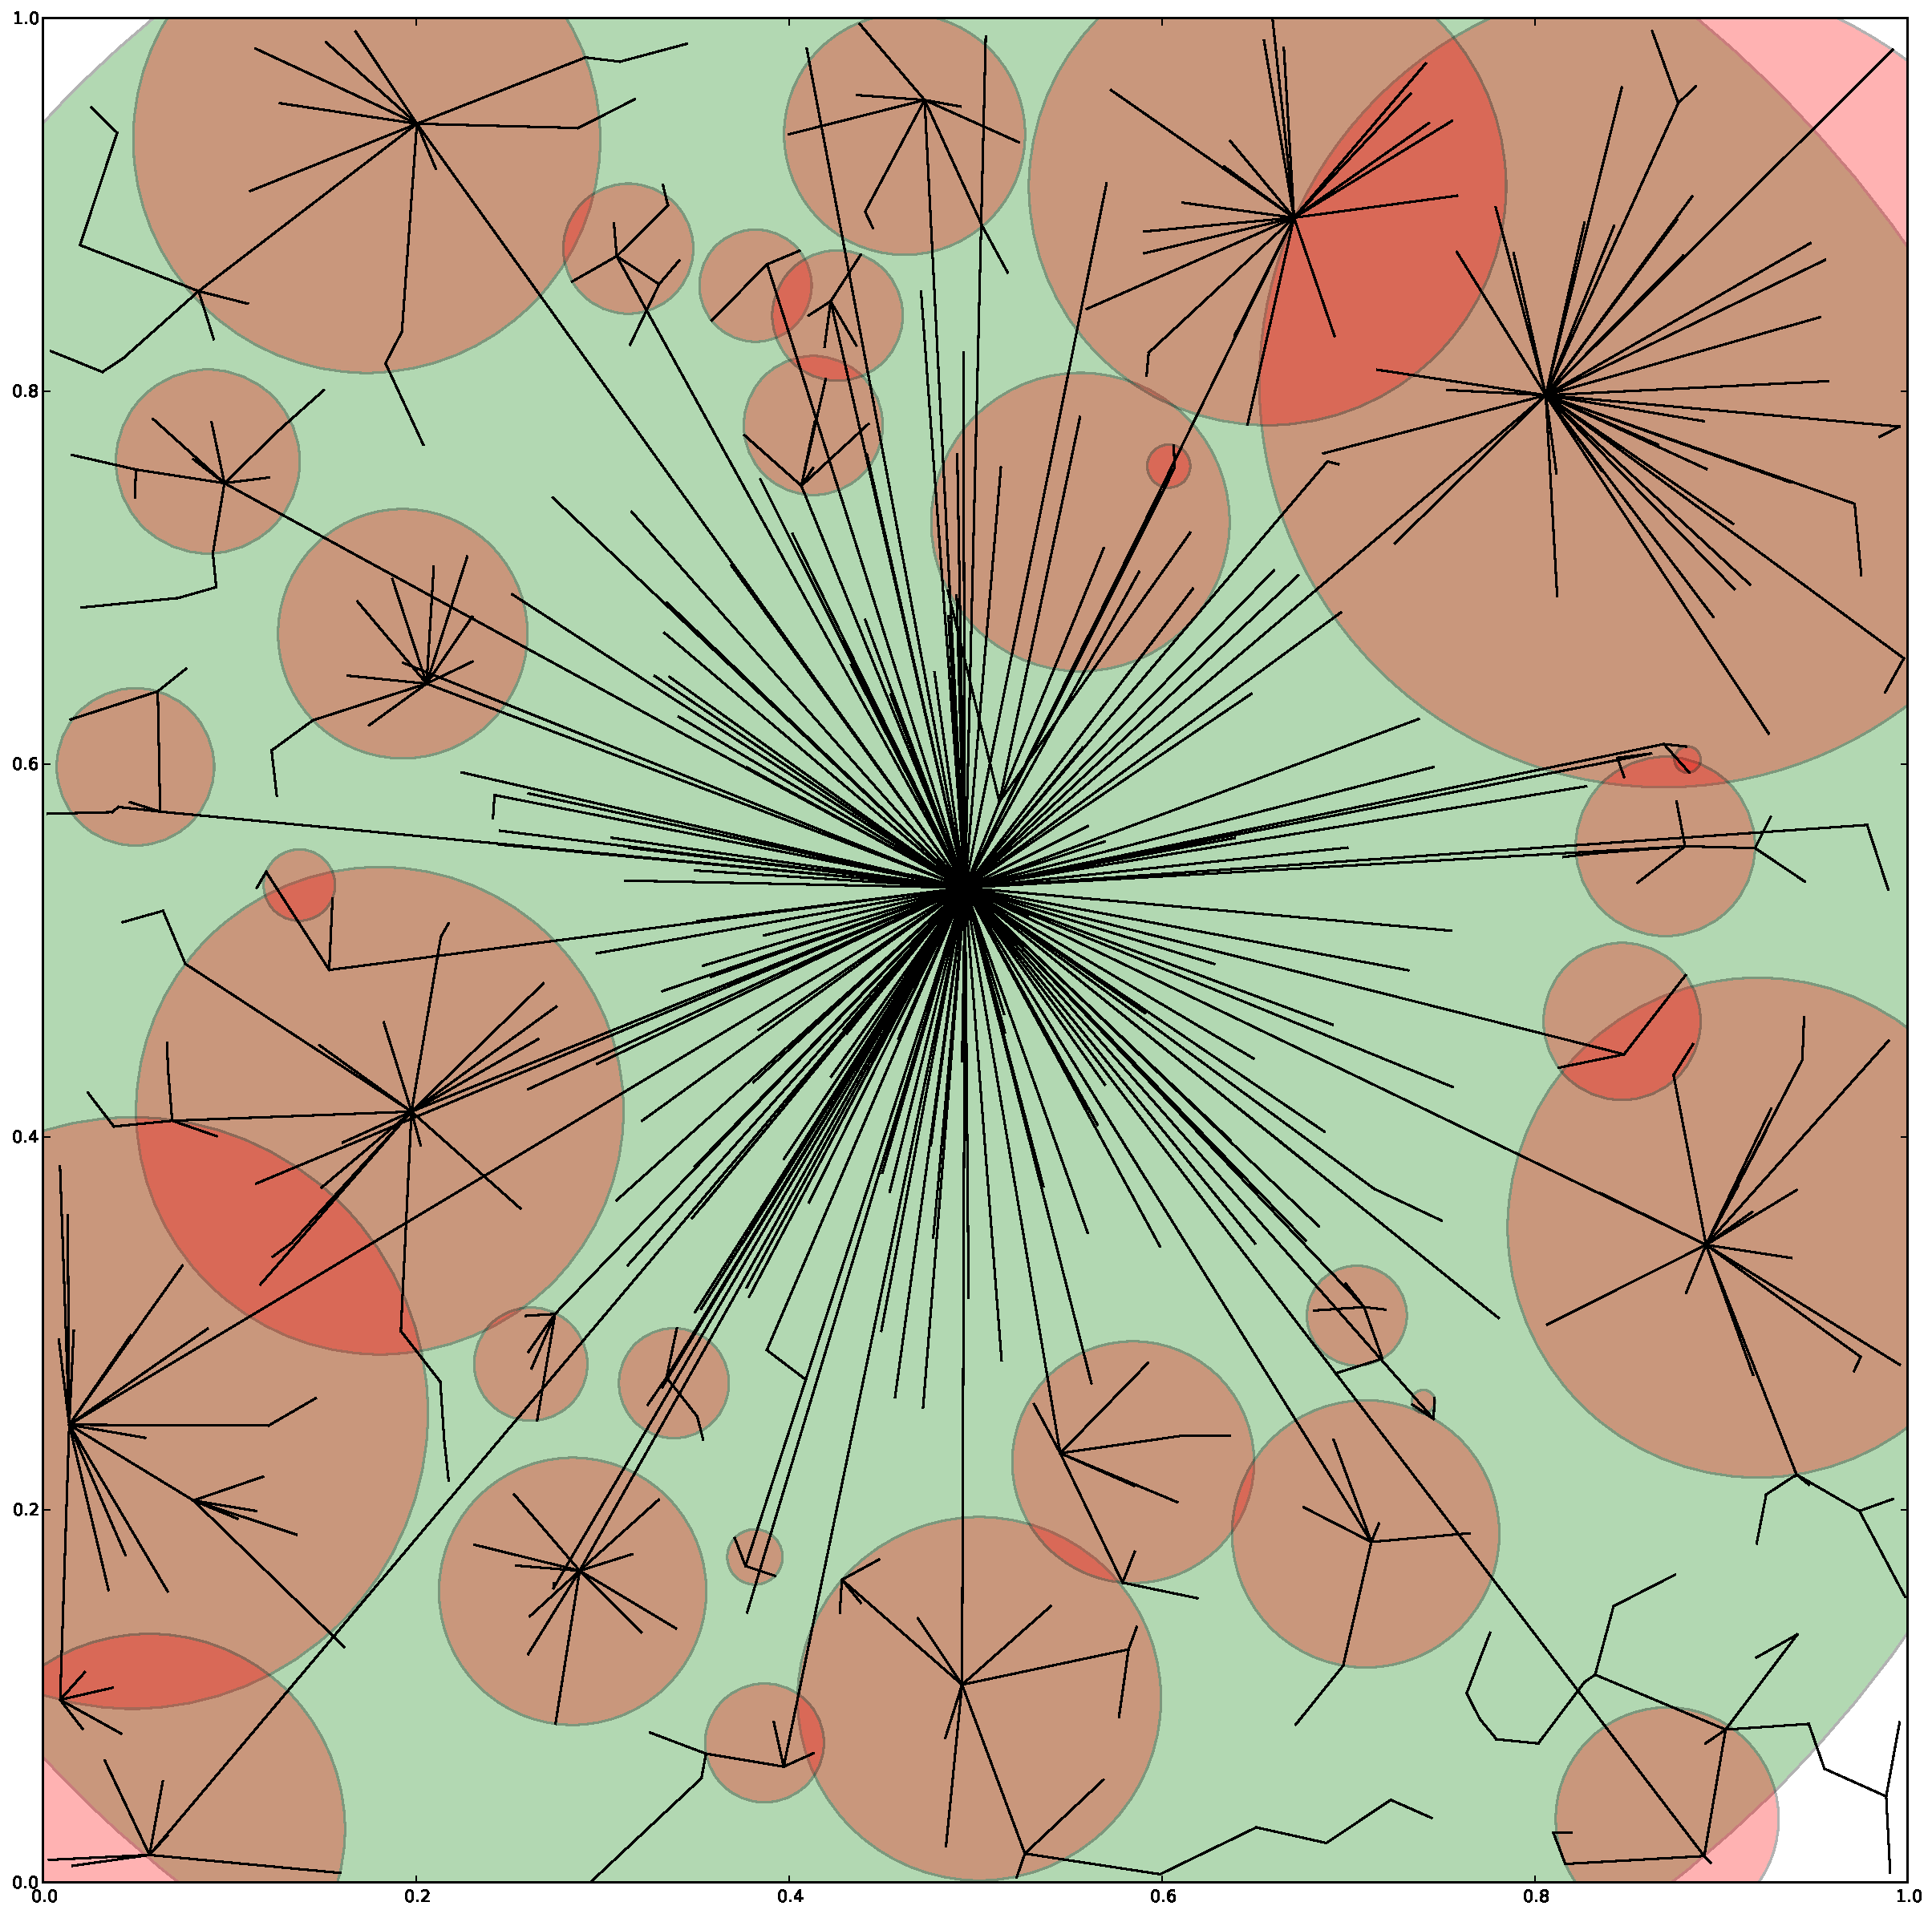
\includegraphics[width=0.65\textwidth]{gfx/chapter-networks/figure4.pdf} 
    \caption{{\bf Influence zones.} Example of a graph where we represent the influence zones for the
first two hierarchical levels.\label{fig:separation_example}} \end{figure}

\subsection{Distance between hierarchical levels}
 
We propose here a quantitative characterisation of the part (1) in the
definition of spatial hierarchy. The first step is to identify the root of the
network which allows us to naturally characterize a hierarchical level by its
topological distance to the root. We choose the most populated node as the root
(which will be the largest hub for $\beta\ll\beta^*$) and we can now measure
various quantities as a function of the level in the hierarchy. In
Fig.~\ref{fig:distance_hierarchy}, we plot the average euclidean distance
$\overline{d}$ between the different hierarchical levels as a function of the
topological distance from the root node (for the sake of clarity, we also draw
next to these plots the corresponding graphs). For reasonably small  values of
$\beta/\beta^*$ (i.e. when the graph is not far from being a star-graph), the
average distance between levels decreases as we go further away from the root
node. This confirms the idea that the graphs for $\beta/\beta^*\simeq 1$ exhibit
a spatial hierarchy where nodes from different levels are getting closer and
closer to each other as we go down the hierachy. Eventually, as $\beta/\beta^*$
becomes larger than 1, the distance between consecutive levels just fluctuates
around $\ell_1\sim 1/\sqrt{\rho}$ the average distance between nearest
neighbours for a Poisson process, which indicates the absence of hierarchy in
the network.



\subsection{Geographical separation of hubs zones} 

We now discuss the part (2) of the definition of spatial hierarchy, that is to
say how the hubs are located in space. Indeed, another property that we can
expect from spatially hierarchical graph is that of \emph{geographical
separation}.


\subsubsection{Separation}
\label{ssub:separation}

We say that a graph is geographically separated if the influence zones of every
node of a given hierarchical level do not overlap and if they are included in
the influence zone of the nodes of the previous level in the hierarchy.
Formally, if we designate by $\mathcal{I}^i_l$ the influence zone of the node
$i$ located at level $l$ in the hierarchy, $\mathcal{I}_l = \cup_{i \in l}
\mathcal{I}^i_l$ the reunion of all the influence zones for nodes belonging to
the level $n$. We say that the graph is geographically separated if:

\begin{align}
    &\mathcal{I}_l \subset \mathcal{I}_{l+1} \; \forall l\\
    &\mathcal{I}^i_l \cap \mathcal{I}^j_l = \O \; \text{if} \; j \neq i, \forall l
\end{align}

The degree of geographical separability of a graph strongly depends on the
definition of the influence zone of a node. For instance, if we take the
influence zone of a node $i$ to be the surface of smallest area containing all
the nodes connected to $i$, it follows that all planar graph are totally
separated.  In the context of transportation networks, we expect hubs to radiate
up to a certain distance around them, that is to say connect to all the nodes
located in a convex shape. We simply define the influence zone of a node $i$ as
the circle centered on the barycenter of i's neighbours that belong to the next
level, of radius the maximum distance between the barycenter and those points. 

Figure~\ref{fig:separation_example} is intended to help the reader visualise
these influence zones on an example: The green circle represent the influence
zone of the root and the red circles the influence zones of the hubs connected
to it. One can see that the graph is geographically separated up to a good
approximation.

\begin{figure}
    \centering
    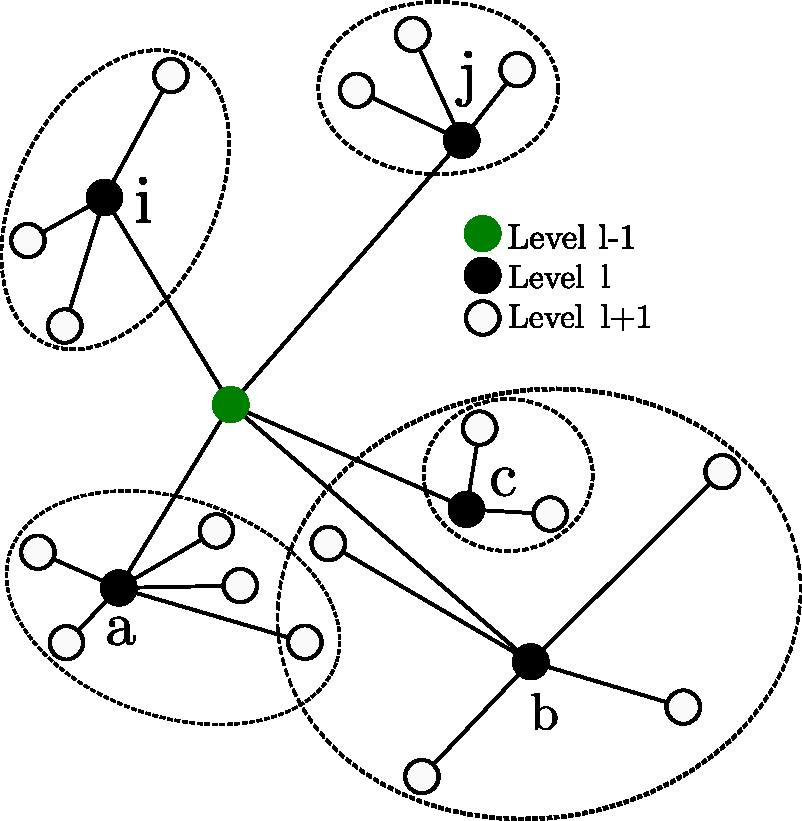
\includegraphics[width=0.45\textwidth]{gfx/chapter-networks/figure10.pdf}\\
    \caption{{\bf Influence zones.} Illustration of the influence zones (dotted
    lines) around several hubs. We have, according to the definition of the
separation index, $S(i,j)=0$, $0 < S(a,b)< 1$ and $S(b,c)=1$.
\label{fig:separation_illustration}} 
\end{figure}

In order to quantify this notion of geographical separability, we define the
separation index of the level $l$ as the average over all the nodes belonging to
$l$ of the separation function. The separation function is equal to $1$ if the
distance $d(i,j)$ between the centers of the influence zones of $i$ and $j$ is
larger than their respective radius (no overlap), and equal to 

\begin{equation}
    S(i,j) = 1-\frac{\text{Area of the overlap between} \; \mathcal{I}_l^i \; \text{and} \; \mathcal{I}_l^j}{\min \left(\text{Area of} \; \mathcal{I}_l^i\text{, Area of} \; \mathcal{I}_l^j\right)}
\end{equation}

One can see that the separation function is equal to 1 if the nodes' influence
zones do not overlap at all and 0 if they perfectly overlap (all the influence
zones overlapping, like Russian dolls). Therefore, the separation index is equal
to 1 if the level s is perfectly separated and 0 if the influence zones are
completely mixed. One can see on Fig.~\ref{fig:separation_illustration} an
illustration expliciting the value of the separation index for different
situations.

\subsubsection{Geographical separation in the intermediate regime}
\label{ssub:geographical_separation_of_simulated_graphs}

We plot the separation index averaged over the all the graph's levels for
different values of $\beta/\beta^*$ on Fig.~\ref{fig:separation}. One can
observe on this graph that the separation index reaches values above $0.90$ when
$\beta/\beta^* \geq 1$, which means that the corresponding graphs indeed have a
structure with hubs controlling geographically well-separated regions.
Obviously, the choice of the shape of the influence zone (which is chosen here
to be a disk) strongly impacts the results but the
same qualitative behavior will be obtained for any type of convex shapes.

\begin{figure}
    \centering
    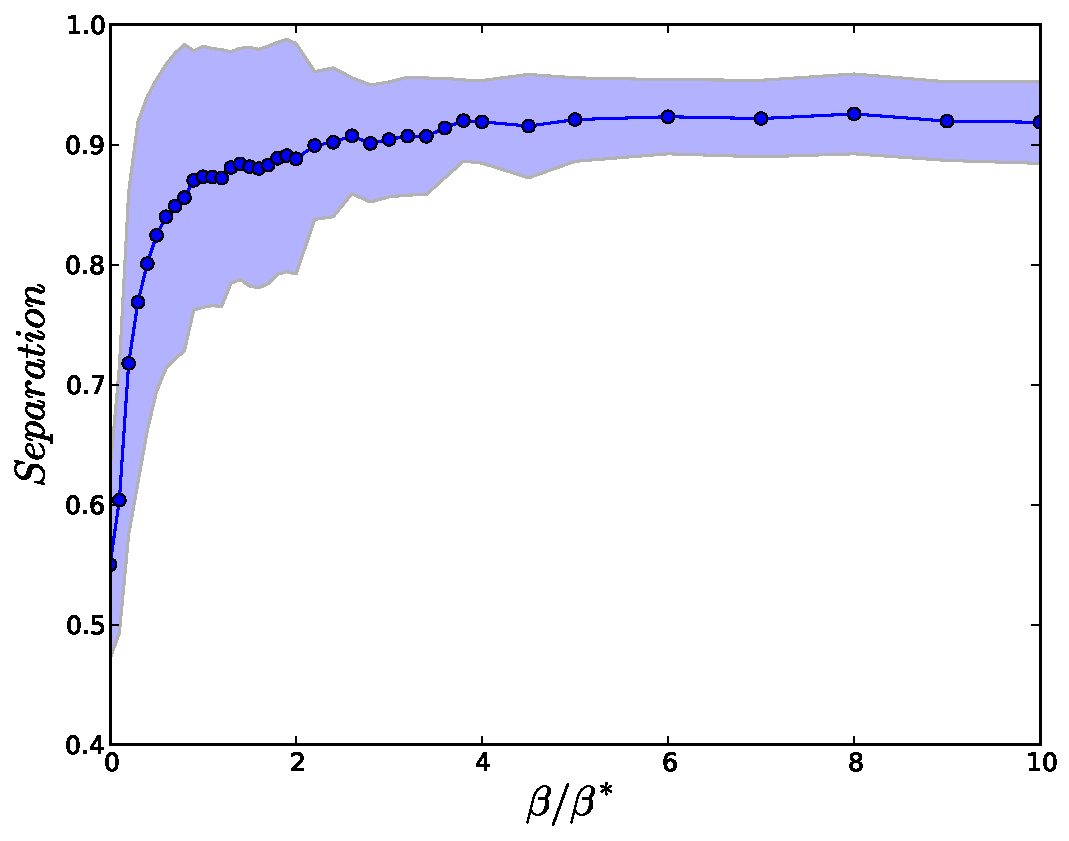
\includegraphics[width=0.80\textwidth]{gfx/chapter-networks/figure6.pdf}
    \caption{{\bf Separation index.} Separation index averaged over all the graph's level versus
$\beta/\beta^*$. The shaded area represents the standard deviation.
\label{fig:separation}} 
\end{figure}

In conclusion, the graphs produced by our model in the regime $\beta / \beta^*$
satisfy the two points of the definition. They exhibit a spatially hierarchical
structure, characterised by a distance ordering and geographical separation of
hubs. We saw earlier that in this regime we have specific, non trivial
properties such as $L_{tot}$ scaling with an exponent depending continuously on
$\beta/\beta^*$. Using a simple toy model, we will now show that the spatial
hierarchy can explain this property.

\subsection{Understanding the scaling with a hierarchical model} 

The exponents $1$ and $0.5$ for the scaling for $L_{tot}$ with the total number
of nodes $N$ is well-understood. However, it is not clear how we can obtain
intermediate values. In the following we show with a simplified model that spatial
hierarchy can indeed lead to scaling exponents in the range $\left[0.5,
1\right]$. We consider the toy model defined by the fractal tree depicted on
Fig.~\ref{fig:fractal_network} for which the distance between the levels $n$ and
$n+1$ is given by

\begin{figure}
    \centering
    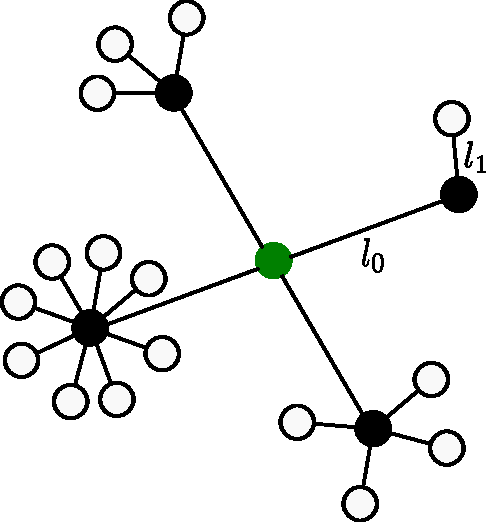
\includegraphics[width=0.60\textwidth]{gfx/chapter-networks/figure7.pdf}
    \caption{{\bf Fractal toy model.} A schematic representation of the hierarchical fractal network used as a toy model. 
    \label{fig:fractal_network}}
\end{figure}

\begin{equation}
    \ell_n=\ell_0 b^n
    \label{eq:fractal_distance}
\end{equation}

where $b\in [0,1]$ is the scaling factor. Each node at the level $n$ is
connected to $z$ nodes at the level $n+1$ which implies that

\begin{equation}
    N_n = z^n
    \label{eq:fractal_nodes}
\end{equation}

where $z>0$ is an integer. A simple calculation on this graph shows that in the
limit $z^g \gg 1$, the total length of the graph with g levels scales as

\begin{equation}
    L_{tot} \sim N^{\frac{\ln(b)}{\ln(z)}+1}
\end{equation}

where $\frac{\ln(b)}{\ln(z)} +1 \leq 1$ because $b \leq 1$ and $z>1$. This
simple model thus provides a simple mechanism accounting for continuous values
of $\tau$ whose value depends on the scaling factor $b$. It provides a
simplified picture of the graphs in the intermediate regime $\beta \simeq
\beta^*$ and exhibits the key features of the graphs in this regime: the hub
structure reminiscent of the star graph and where the nodes connected to each
hub form geographically distinct regions, organized in a hierarchical fashion.
It is also interesting to note that the parameter $z$ can be easily determined
from the average degree of the network, and that the parameter $b$ of the toy
model can be related to our model by measuring the decrease of the mean distance
between different levels of the hierarchy, as in
Fig.~\ref{fig:distance_hierarchy}. By plotting these curves for different values
of $\beta/\beta^*$, we find that the coefficient of the exponential decays
decreases linearly with $\beta / \beta^*$ and therefore that $b \sim
e^{\beta/\beta*}$ (However, the comparison only makes sense in the regime $\beta
\sim \beta^*$, as otherwise the graphs do not exhibit spatial hierarchy).

\begin{figure}
    \centering
    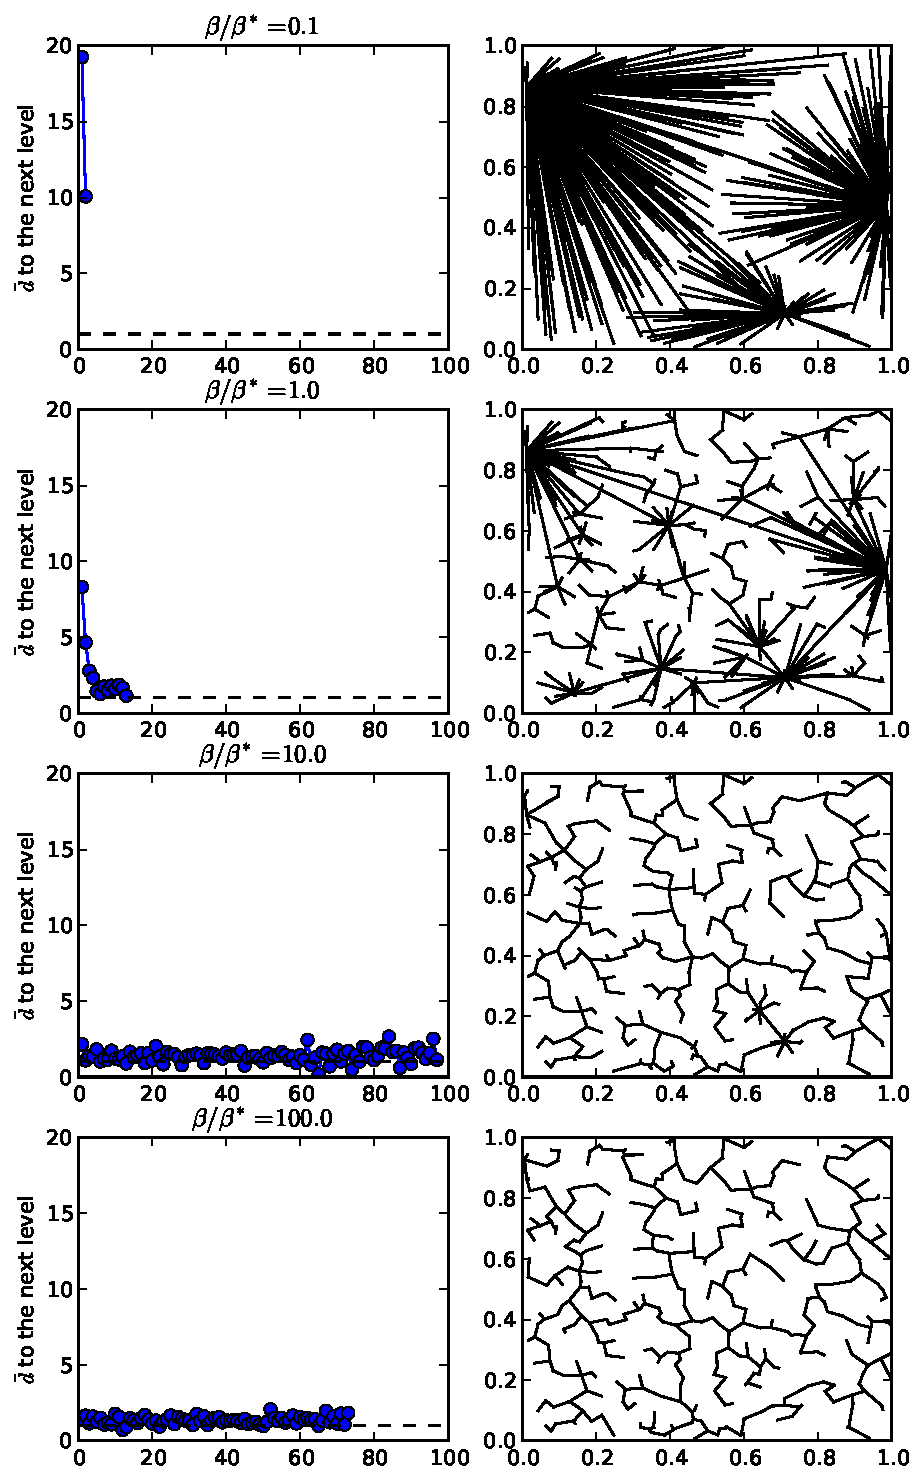
\includegraphics[width=0.80\textwidth]{gfx/chapter-networks/figure5.pdf}
    \caption{{\bf Distance between hierarchy levels.} Left column: Average
    distance between the successive hierarchy levels for different values of
    $\beta/\beta^*$, next to the corresponding graphs (on the right column). The
    most populated node is taken as the root node. \label{fig:distance_hierarchy}}
\end{figure}




\section{Efficiency}

Most transportation networks are not obtained by a global optimization but
result from the addition of various, successive layers. The question of the
efficiency of these self-organized systems is therefore not trivial and deserves
some investigation. The model considered here allows us to test the effect of
various parameters and how efficient a self-organized system can be. In
particular, we would like to characterize the efficiency of the system for
various values of $\beta$. For this, we can assume that the construction cost
per unit length is fixed (ie. the factor $\eta$ in Eq.~\ref{eq:cost} is
constant), and since $\beta = \frac{\eta}{\kappa}$ a change of value for $\beta$
is equivalent to a change in the benefits per passenger per unit of length. 

A first natural measure of how optimal the network is, is given by its total
cost proportional to the total length $L_{tot}$: the shorter a network is, the
better for the company in terms of building and maintenance costs. In our model,
the behaviour of the total cost is simple and expected: for small values of
$\beta/\beta^*$, the obtained networks correspond to a situation where the users
are charged a lot compared to the maintenance cost, and the network is very long
($L_{tot}\propto N$). In the opposite case, when $\beta/\beta^* \gg 1$ the main
concern in building this network is concentrated on construction cost and the
network has the smallest total length possible (for a given set of nodes). 

The cost is however not enough to determine how efficient the network is from
the users' point of view: a very low-cost network might indeed be very
inefficient. A simple measure of efficiency is then given by the amount of
detour needed to go from one point to another. In other words, a network is
efficient if the shortest path on the network for most pairs of nodes is very
close to a straight line. The detour index for a pair of nodes $(i,j)$ is
conveniently measured by $D(i,j)/d(i,j)$ where $D(i,j)$ is the length of the
shortest path between $i$ and $j$, and $d(i,j)$ is the euclidean distance
between $i$ and $j$. In order to have a detailed information about the network,
we use the quantity introduced in~\cite{Aldous:2010}

\begin{equation}
    \phi(d) = \frac{1}{\mathcal{N}(d)} \sum_{\substack{i,j\\d(i,j) =d}} \frac{D(i,j)}{d(i,j)}
\end{equation}

where the normalisation $\mathcal{N}(d)$ is the number of pairs with $d(i,j)=d$.
We plot this `detour function' for several values of $\beta/\beta^*$ on
Fig.~\ref{fig:RLE}(A). For $\beta/\beta^* \ll 1$, the function $\phi(d)$ takes
high values for $d$ small and low values for large $d$, meaning that the
corresponding networks are very inefficient for relatively close nodes while
being very efficient for distant nodes. On the other hand, for $\beta/\beta^*
\gg 1$ we see that the MST is very efficient for neighboring nodes but less
efficient than the star-graph for long distances. Surprisingly, the graphs for
$\beta/\beta^* \sim 1$ exhibit a non trivial behaviour: for small distances, the
detour is not as good as for the MST, but not as bad as for the star graph and
for long distances it is the opposite. In order to make this statement more
precise we compute the average of $\phi(d)$ over $d$ (a quantity which has a
clear meaning for trees, see~\cite{Aldous:2010} for objections to the use of $<
\phi(d) >$ as a good efficiency measure in general), and plot it as a function
of $\beta/\beta^*$. The results are shown in Fig.~\ref{fig:RLE}(B) and confirm
this surprising behavior in the intermediate regime: we observe a minimum for
$\beta/\beta^* \sim 1$. In other words, there exists a non trivial value of
$\beta$, i.e. a value of the benefits per passenger per unit of length, for
which the network is optimal from the point of view of the users. 

\begin{figure}
    \centering
    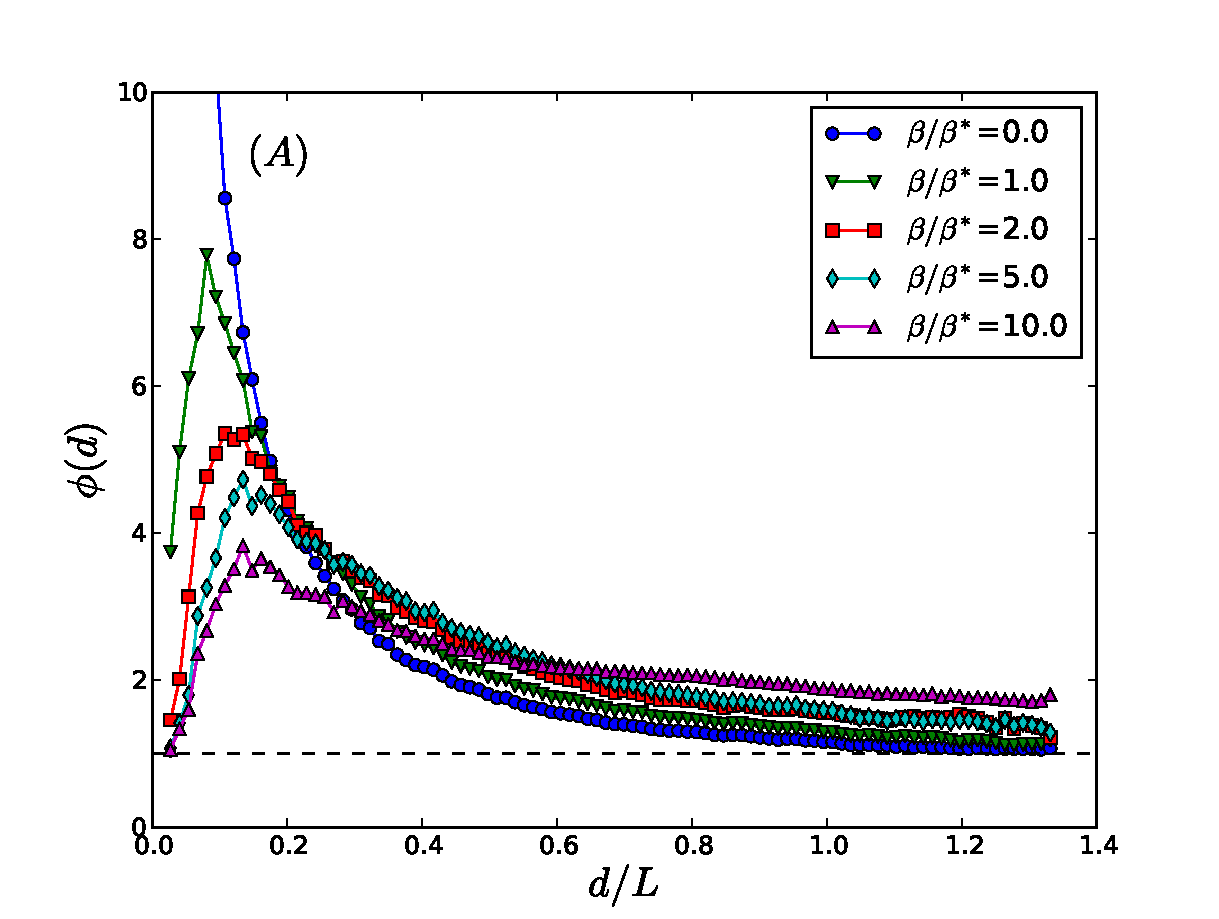
\includegraphics[width=0.49\textwidth]{gfx/chapter-networks/figure8a.pdf}
    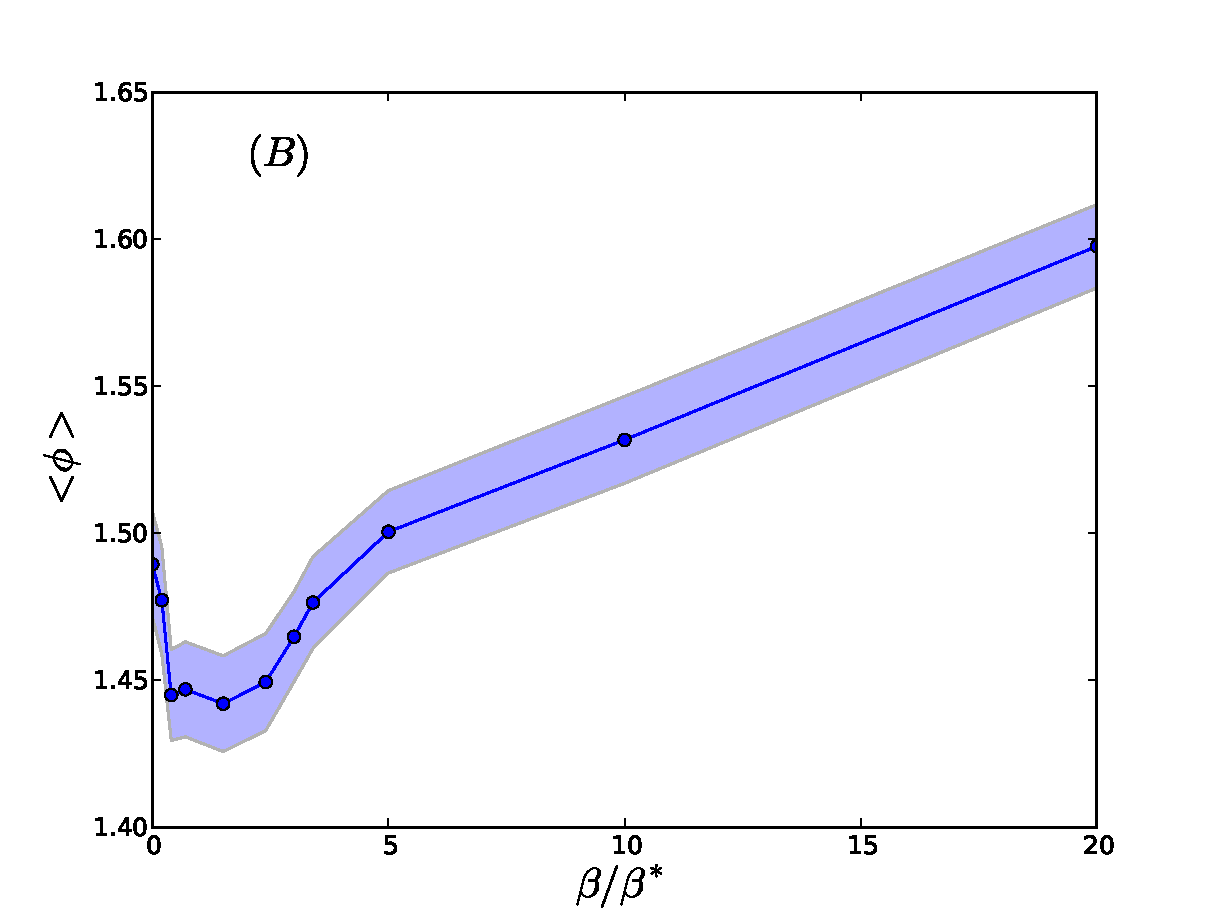
\includegraphics[width=0.49\textwidth]{gfx/chapter-networks/figure8b.pdf}
    \caption{{\bf Detour function.} (Left) Detour function $\phi (d)$ versus the
        relative distance between nodes for different values of $\beta/\beta^*$.
        (Right) Average detour index $< \phi >$  for several realisations of the
        graphs as a function of $\beta/\beta^*$. The shaded area represents the
        standard deviation of $< \phi >$. This plot shows that there is a
        minimum for this quantity in the intermediate regime $\beta\sim\beta^*$.
\label{fig:RLE}} 
\end{figure}

The existence of such an optimum is far from obvious and in order to gain more
understanding about this phenomenon, we plot the Gini coefficient $G_l$ relative
to the length of the edges between nodes in Fig.~\ref{fig:gini_length}. We
observe that the Gini coefficient peaks around $\beta/\beta^* = 1$, which means
that in this regime, the diversity in terms of edge length is the highest. The
large diversity of lengths explains why the network is the most efficient in
this regime: indeed long links are needed to cover large distances, while
smaller links are needed to reach efficiently all the nodes. It is interesting
to note that this argument is similar to the one proposed by Kleinberg
\cite{Kleinberg:2000} in order to explain the existence of an optimal delivery
time in small-world networks.

\begin{figure}
    \centering
    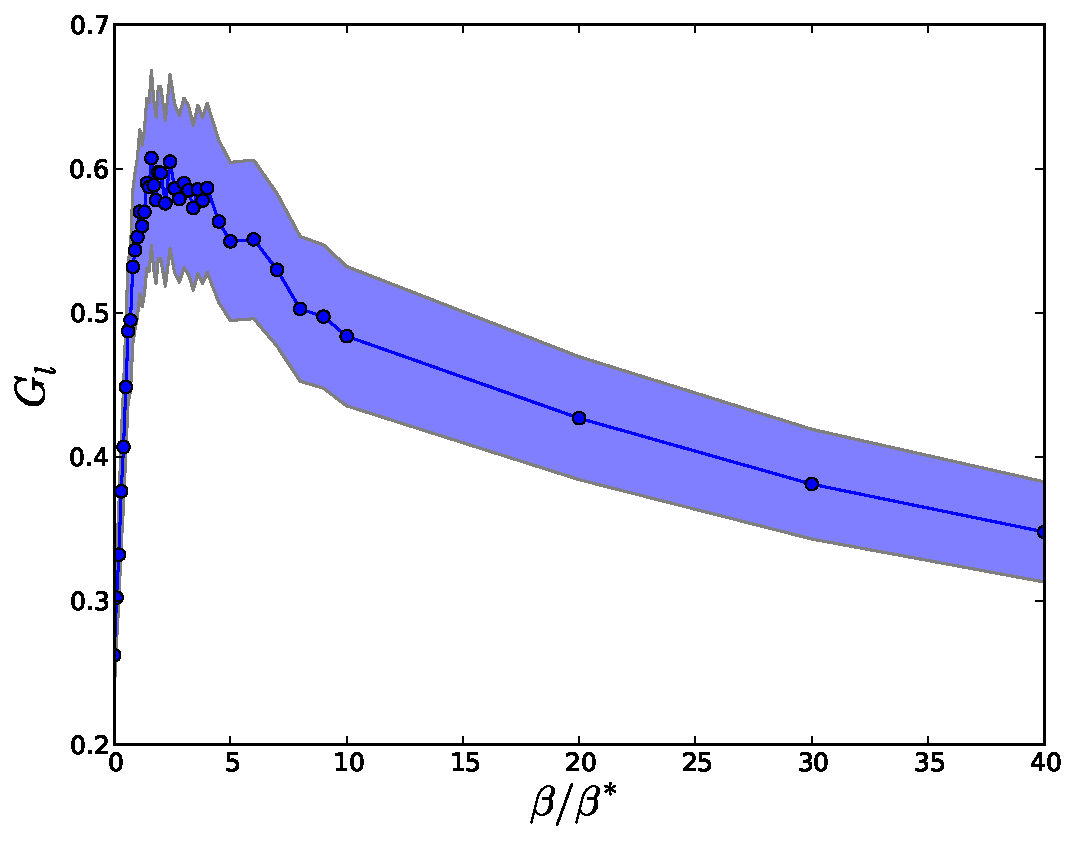
\includegraphics[width=0.8\textwidth]{gfx/chapter-networks/figure9.pdf}
    \caption{{\bf Gini on the length.} Evolution of the Gini coefficient for the length versus $\beta/\beta^*$ (for different values of $\beta^*$). The shaded area represents the standard deviation. \label{fig:gini_length}}
\end{figure}


\section{Discussion}

We have presented a model of a growing spatial network based on a cost-benefit
analysis. This model allows us to discuss the effect of a local optimization on
the large-scale properties of these networks. First, we showed that the graphs
exhibit a crossover between the star-graph and the minimum spanning tree when
the relative importance of the cost increases. This crossover is characterized
by a continuously varying exponent which could give some hints about other
quantities observed in cities such as the total length travelled by the
population. Secondly, we showed that the model predicts the emergence of a
spatial hierarchical structure in the intermediate regime where costs and
benefits are of the same order of magnitude. We showed that this spatial
hierarchy can explain the non trivial behaviour of the total length versus the
number of nodes. Finally, this model shows that in the intermediate regime the
vast diversity of links lengths entails a large efficiency, an aspect which
could of primary importance for practical applications.

An interesting playground for this model is given by railways and we can
estimate the value of $\beta/\beta^*$ for these systems. In some cases, we were
able to extract the data from various sources (in particular financial reports
of railway companies) and the results are shown in Table~1. We estimate for
different real-world networks, including some of the oldest railway systems,
$\beta$ using its definition (total maintenance costs per year divided by the
total length and by the average ticket price per km). In order to estimate
$\beta^*$ we use Eq.\ref{eq:beta*_traffic} in the following way

\begin{equation}
    \beta^*\simeq\frac{T_{tot}}{L_{tot}}
\end{equation}

where $T_{tot}$ is the total travelled length (in passengers$\cdot$kms$/$year)
and $L_{tot}$ is the total length of the network under consideration.
Remarquably, the computed values for the ratio $\beta/\beta^*$ shown in
Table~\ref{table:b_b*}.
are all of the order of $1$ (ranging from $0.20$ to $1.56$). In the framework of
this model, this result shows that all these systems are in the regime where the
networks possess the property of spatial hierarchy, suggesting it is a crucial
feature for real-world networks. We note that in our model, the value of $\beta
/ \beta^*$ is given exogeneously, and it would be extremely interesting to
understand how we could construct a model leading to this value in an
endogeneous way.

\begin{table*}
\scalebox{0.8}{
\begin{tabular}{lcccccc}
%\begin{tabular}{@{\vrule height 10.5pt depth4pt  width0pt} lccccccc}
\hline
Country & $T_{tot}$ & $L_{tot}$ & Maintenance & Ticket price & $\beta/\beta^*$ \\
 & \footnotesize(kms$/$year) & \footnotesize(kms) & \footnotesize(euros$/$year)
& \footnotesize{euros} &  \\
\hline
France & $88.1 \, 10^9$ & $29,901$	&	$2.10 \, 10^9 $ & $0.12$ & $\mathbf{0.20}$ \\
Germany & $79.2 \, 10^9$ & $37,679$	&	$7.50 \, 10^9 $ & $0.30$ & $\mathbf{0.32}$ \\
India & $978.5 \, 10^9$ & $65,000$	& 	$3.00 \, 10^9 $ & $0.01$ & $\mathbf{0.31}$ \\
Italy & $40.6 \, 10^9$ & $24,179$	& 	$4.30 \, 10^9 $ & $0.20$ & $\mathbf{0.53}$ \\
Spain & $22.7 \, 10^9$ & $15,064$	& 	$3.16 \, 10^9 $ & $0.11$ & $\mathbf{1.26}$ \\
Switzerland & $18.0 \, 10^9$ & $5,063$	& 	$2.03 \, 10^9 $ & $0.17$ & $\mathbf{0.66}$ \\
United Kingdom & $62.7 \, 10^9$ & $16,321$	&	$12 \, 10^9 $ & $0.16$ & $\mathbf{1.19}$ \\
United States & $17.2 \, 10^9$ & $226,427$	& 	$2.96 \, 10^9 $ & $0.11$ & $\mathbf{1.56}$\\
\hline
\end{tabular}
}
\caption{{\bf Empirical estimates for $\beta / \beta^*$}. Table giving the total
ride distance (in km), the total network length (in km), the total annual
maintenance expenditure (in euros per year)  and the average ticket price (in
euros per km). All the given values correspond to the year 2011. From these data
we compute the experimental values of $\beta$, $\beta^*$ and their ratio (data
obtained from various sources such as financial reports of railway companies)
\label{table:b_b*}} \end{table*}

There are also several directions that seem interesting. First, various forms of
cost and benefits functions could be investigated in order to model specific
networks. In particular, there are several choices that can be taken for the
expected traffic. In this paper we limited ourselves to estimate the traffic as
a direct traffic from a node $i$ to a node $j$, but it is likely that part of
the traffic will come from other nodes. In order to take this into account, we
think that the following extensions are probably interesting:

\begin{enumerate}
    \item A given city (denoted by $0$ with population $M_0$) plays a particular role in the network (the capital city in a relatively small country, for example). In that case it is beneficial to be close to that city through the network and we write
    \begin{equation}
        \label{eq:R1}
        R^{(1)}_{ij} = (1-\lambda)\frac{M_i M_j}{d_{ij}^{a-1}}  + \lambda \: \frac{M_i M_0}{\left(D_{0j} + d_{ij}\right)^{a-1}}- \beta \: d_{ij}
    \end{equation}
    where $\lambda \in \left[ 0,1 \right]$ is a coefficient weighing the relative importance of the traffic coming from the particular city.

    \item The most general case where all the network-induced traffic are taken into account. We then consider
    \begin{equation}
        \label{eq:R2}
        R^{(2)}_{ij} = \sum_{k \neq i}\frac{M_i M_k}{\left(D_{kj} + d_{ij}\right)^{a-1}}- \beta \: d_{ij}
    \end{equation}
\end{enumerate} 

Other ingredients such as the presence of different rail companies, or the
difference between a state-planned network and a network built by private
actors, etc, could easily be implemented and the corresponding models could
possibly lead to interesting results.

More importantly, we limited ourselves here to trees in order to focus on the
large-scale consequences of the cost-benefit mechanism. Further studies are
needed in order to uncover the mechanisms of formation of loops in growing
spatial networks and we believe that the model presented here might represent a
suitable modeling framework.

Finally, it seems plausible that the general cost-benefit framework introduced
at the beginning of the article could be applied to the modelling of systems
besides transportation networks. We believe it captures the fundamental features
of spatial network while being versatile enough to model the growth of a great
diversity of systems shaped by space.
